 \سؤال{ایجاد \lr{pipe} یک‌سویه}
 
\begin{enumerate}
 	\item برای ساخت ارتباط یک‌سویه از دستور و فراخوانی سیستمی \lr{pipe} استفاده می‌شود.
 	
 	\begin{figure}[!hbpt]
 		\centering
 		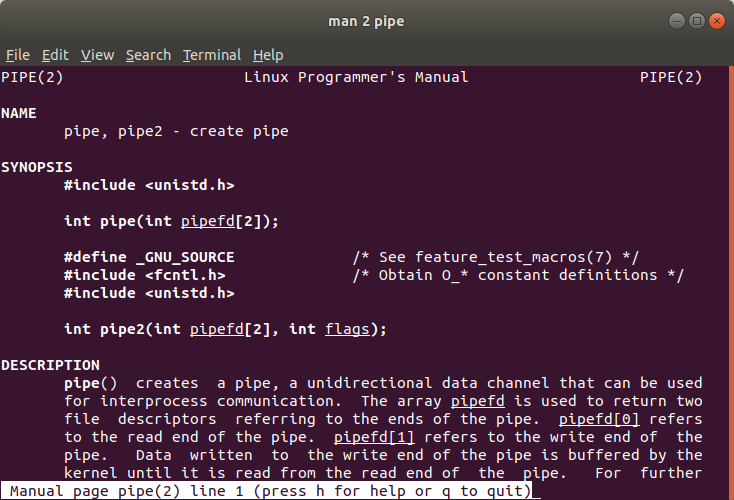
\includegraphics[scale=0.5]{./img/pipe.png}
 		\caption{عمل‌کرد \lr{pipe}}
 	\end{figure}
 	\item 
 	همان‌طور که در مستند جلسه‌ی پنجم توضیح داده شده است، برای ساخت یک \lr{pipe} جدید کافی است به‌صورت زیر عمل کنیم:
	\begin{Verbatim}[tabsize=4]
#include <stdio.h>
#include <stdlib.h>
#include <unistd.h>


int main()
{
	int pipefd[2];
	int result = pipe(pipefd);
	if (result == 0)
	{
	printf("pipe done");
	}
	return 0;
}
 	\end{Verbatim}
	\item 
	برای انتقال پیام \lr{Hello world!} از پدر به فرزند و چاپ آن در خروجی باید کد زیر را اجرا کنیم:


	\begin{Verbatim}[tabsize=4]
#include <stdio.h>
#include <stdlib.h>
#include <unistd.h>

#define MSG_SIZE 11


int main()
{
	int pipefd[2];
	int result = pipe(pipefd);
	if (fork() > 0)
	{
		printf("parent is executed...\n");
		close(pipefd[0]);
		printf("writing message in the file descriptor...\n");
		write(pipefd[1], "Hello world", MSG_SIZE);
		printf("closing read file descriptor in parent...\n");
		close(pipefd[1]);
	}
	else {
		char msg[MSG_SIZE];
		printf("child is executed...\n");
		read(pipefd[0], msg, MSG_SIZE);
		printf("%s", msg);
	}
	return 0;
}
	\end{Verbatim}
	

	\item در این قسمت می‌خواهیم	 خروجی پردازه‌ی پدر (دستور \lr{ls}) را به عنوان ورودی به پردازه‌ی فرزند بدهیم.
	
	\begin{Verbatim}[tabsize=4]
#include <stdio.h>
#include <stdlib.h>
#include <unistd.h>

int main(int argc, char **argv)
{
	int pipefd[2];
	pipe(pipefd);
	
	if (fork() > 0)
	{
		close(pipefd[0]);
		dup2(pipefd[1], STDOUT_FILENO); //make output go to the pipe
		execlp("ls", "ls", "-a", (char *) NULL);
	}
	
	close(pipefd[1]);
	dup2(pipefd[0], STDIN_FILENO); //get input from pipe
	execlp("wc", "wc",(char *) NULL);
}
	\end{Verbatim}
	\item برای ایجاد ارتباطات تمام دو طرفه بین پردازه‌ها باید دو بار از \lr{pipe} استفاده کرد. به کمک یکی از آن‌ها در یکی بخوانیم و به کمک دیگری بنویسیم.
	
	\begin{Verbatim}[tabsize=4]
#include <stdio.h>
#include <stdlib.h>
#include <string.h>
#include <unistd.h>

int main(void)
{
	int pid, n, c, p, k, nbread;
	char buf1[12], buf2[12];
	int fd1[2], fd2[2];
	pipe(fd1);
	pipe(fd2);
	pid = fork();
	if (pid == 0)
	{
		close(fd1[1]);
		close(fd2[0]);
		read(fd1[0], buf2, sizeof(buf2));
		n = atoi(buf2);
		printf("Child read %d\n", n);
		for (int i = 0; i < n; i++)
		{
			printf("child dozes...\n");
			sleep(3);
			printf("child wakes...\n");
			nbread = read(fd1[0], buf2, sizeof(buf2));
			if (nbread == -1)
			{
				fprintf(stderr, "child exits after read failure\n");
				exit(1);
			}
			c = atoi(buf2);
			c = c * 2;
			sprintf(buf2, "%d", c);
			write(fd2[1], buf2, sizeof(buf2));
			printf("Child wrote [%s]\n", buf2);
		}
		close(fd1[0]);
		close(fd2[1]);
		printf("Child done\n");
		exit(0);
	}
	else
	{
		close(fd1[0]);
		close(fd2[1]);
		printf("Enter integer: ");
		scanf("%d", &p);
		sprintf(buf1, "%d", p);
		write(fd1[1], buf1, sizeof(buf1));
		printf("Parent wrote [%s]\n", buf1);
		printf("parent dozes...\n");
		sleep(3);
		printf("parent wakes...\n");
		for (int i = 0; i < p; i++)
		{
			sprintf(buf1, "%d", i);
			write(fd1[1], buf1, sizeof(buf1));
			printf("parent wrote [%s]\n", buf1);
			read(fd2[0], buf2, sizeof(buf2));
			printf("number is: %s\n", buf2);
		}
		close(fd1[1]);
		close(fd2[0]);
		wait(NULL);
	}
	return 0;
}
	\end{Verbatim}
\end{enumerate}
	
\newpage

\سؤال{سیگنال‌ها}

\begin{enumerate}
	\item در این قسمت با استفاده از دستور \lr{man 7 signal} اطلاعات راجع به این فراخوان سیستمی را می‌توانیم مشاهده کنیم.
	\begin{figure}[!hbpt]
		\centering
		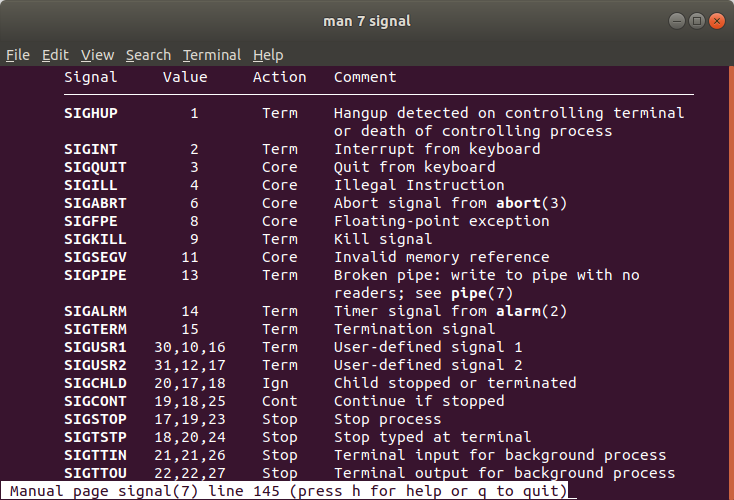
\includegraphics[scale=0.5]{./img/signal.png}
		\caption{لیستی از \lr{signal}ها}
	\end{figure}
	\begin{itemize}
		\item \textbf{\lr{SIGINT}}:‌متوقف شدن برنامه از طریق کیبورد را تشخیص می‌دهد.
		\item \textbf{\lr{SIGQUIT}}: از طریق کیبورد از پردازه خارج می‌شود.
		\item \textbf{\lr{SIGTERM}}: سیگنالی است که بیان‌کننده‌ی خاتمه یک پردازه است.
		\item و...
	\end{itemize}
	\item از \lr{alarm()} برای ارسال \lr{SIGALRM} به پردازه استفاده می‌شود. آرگومان اصلی آن زمان است که واحد آن به ثانیه است. اگر مقدار آن صفر باشد، \lr{alarm} خاصی برنامه‌ریزی نمی‌شود.
	\item  کد زیر با توجه به \lr{alarm(5)} ۵ ثانیه اجرا می‌شود و چون داخل حلقه‌ی بی‌نهایت است، بنابراین دیگر خط‌ها (همان‌طور که در \lr{printf} هم مشاهده‌ می‌شود) اجرا نمی‌شوند و برنامه خاتمه پیدا می‌کند.
	\begin{Verbatim}[tabsize=4]
#include <stdio.h>
#include <unistd.h>

int main() 
{
	alarm(5);
	printf("Looping forever...\n");
	while(1);
	printf("This line should never be executed.\n");
	return 0;
}
	\end{Verbatim}
	

	\item تغییر در کد
	\begin{Verbatim}[tabsize=4]
#include <stdio.h>
#include <signal.h>
#include <unistd.h>

int flag = 1; // global flag


void alarm_handler(int signum) {
	flag = 0;
}


int main() 
{
	signal(SIGALRM, alarm_handler); // Register signal handler
	alarm(5);
	printf("Looping forever...\n");
	while(flag){
		pause();
	};
	printf("This line should be executed.\n");
	return 0;
}
	\end{Verbatim}
	\item خروج از برنامه پس از دو بار فشردن کلید ترکیبی \lr{CTRL + C}
	\begin{Verbatim}[tabsize=4]
#include <stdio.h>
#include <signal.h>
#include <unistd.h>
#include <stdlib.h>

int counter = 1; // global flag


void handler(int signum) {
	if (counter == 2){
		printf("\nexiting...\n");
		exit(1);
	}
	else {
		printf("\npress CTRL + C again to exit.\n");
		counter += 1;
	}
}


int main() 
{
	signal(SIGINT, handler);
	while(1);
}
	\end{Verbatim}
\end{enumerate}


